%%%%%%%%%%%%%%%%%%%%%%%%%%%%%%%%%%%%%%%%%
% Programming/Coding Assignment
% LaTeX Template
%
% This template has been downloaded from:
% http://www.latextemplates.com
%
% Original author:
% Ted Pavlic (http://www.tedpavlic.com)
%
% Note:
% The \lipsum[#] commands throughout this template generate dummy text
% to fill the template out. These commands should all be removed when 
% writing assignment content.
%
% This template uses a Perl script as an example snippet of code, most other
% languages are also usable. Configure them in the "CODE INCLUSION 
% CONFIGURATION" section.
%
%%%%%%%%%%%%%%%%%%%%%%%%%%%%%%%%%%%%%%%%%

%----------------------------------------------------------------------------------------
%	PACKAGES AND OTHER DOCUMENT CONFIGURATIONS
%----------------------------------------------------------------------------------------

\documentclass{article}
\usepackage[english]{babel}
\usepackage{amsmath}
\usepackage{fancyhdr} % Required for custom headers
\usepackage{lastpage} % Required to determine the last page for the footer
\usepackage{extramarks} % Required for headers and footers
\usepackage[usenames,dvipsnames]{color} % Required for custom colors
\usepackage{graphicx} % Required to insert images
\usepackage{subcaption}
\usepackage{listings} % Required for insertion of code
\usepackage{courier} % Required for the courier font
\usepackage{lipsum} % Used for inserting dummy 'Lorem ipsum' text into the template

% Margins
\topmargin=-0.45in
\evensidemargin=0in
\oddsidemargin=0in
\textwidth=6.5in
\textheight=9.0in
\headsep=0.25in

\linespread{1.1} % Line spacing

% Set up the header and footer
\pagestyle{fancy}
\lhead{\hmwkAuthorName} % Top left header
\chead{\hmwkClass\ (\hmwkClassTime): \hmwkTitle} % Top center head
%\rhead{\firstxmark} % Top right header
\lfoot{\lastxmark} % Bottom left footer
\cfoot{} % Bottom center footer
\rfoot{Page\ \thepage\ of\ \protect\pageref{LastPage}} % Bottom right footer
\renewcommand\headrulewidth{0.4pt} % Size of the header rule
\renewcommand\footrulewidth{0.4pt} % Size of the footer rule

\setlength\parindent{0pt} % Removes all indentation from paragraphs

%----------------------------------------------------------------------------------------
%	CODE INCLUSION CONFIGURATION
%----------------------------------------------------------------------------------------

\definecolor{MyDarkGreen}{rgb}{0.0,0.4,0.0} % This is the color used for comments
\lstloadlanguages{Perl} % Load Perl syntax for listings, for a list of other languages supported see: ftp://ftp.tex.ac.uk/tex-archive/macros/latex/contrib/listings/listings.pdf
\lstset{language=Perl, % Use Perl in this example
        frame=single, % Single frame around code
        basicstyle=\small\ttfamily, % Use small true type font
        keywordstyle=[1]\color{Blue}\bf, % Perl functions bold and blue
        keywordstyle=[2]\color{Purple}, % Perl function arguments purple
        keywordstyle=[3]\color{Blue}\underbar, % Custom functions underlined and blue
        identifierstyle=, % Nothing special about identifiers                                         
        commentstyle=\usefont{T1}{pcr}{m}{sl}\color{MyDarkGreen}\small, % Comments small dark green courier font
        stringstyle=\color{Purple}, % Strings are purple
        showstringspaces=false, % Don't put marks in string spaces
        tabsize=5, % 5 spaces per tab
        %
        % Put standard Perl functions not included in the default language here
        morekeywords={rand},
        %
        % Put Perl function parameters here
        morekeywords=[2]{on, off, interp},
        %
        % Put user defined functions here
        morekeywords=[3]{test},
       	%
        morecomment=[l][\color{Blue}]{...}, % Line continuation (...) like blue comment
        numbers=left, % Line numbers on left
        firstnumber=1, % Line numbers start with line 1
        numberstyle=\tiny\color{Blue}, % Line numbers are blue and small
        stepnumber=5 % Line numbers go in steps of 5
}

% Creates a new command to include a perl script, the first parameter is the filename of the script (without .pl), the second parameter is the caption
\newcommand{\perlscript}[2]{
\begin{itemize}
\item[]\lstinputlisting[caption=#2,label=#1]{#1.pl}
\end{itemize}
}

%----------------------------------------------------------------------------------------
%	DOCUMENT STRUCTURE COMMANDS
%	Skip this unless you know what you're doing
%----------------------------------------------------------------------------------------

% Header and footer for when a page split occurs within a problem environment
\newcommand{\enterProblemHeader}[1]{
%\nobreak\extramarks{#1}{#1 continued on next page\ldots}\nobreak
%\nobreak\extramarks{#1 (continued)}{#1 continued on next page\ldots}\nobreak
}

% Header and footer for when a page split occurs between problem environments
\newcommand{\exitProblemHeader}[1]{
%\nobreak\extramarks{#1 (continued)}{#1 continued on next page\ldots}\nobreak
%\nobreak\extramarks{#1}{}\nobreak
}

\setcounter{secnumdepth}{0} % Removes default section numbers
\newcounter{homeworkProblemCounter} % Creates a counter to keep track of the number of problems
\setcounter{homeworkProblemCounter}{0}

\newcommand{\homeworkProblemName}{}
\newenvironment{homeworkProblem}[1][Part \arabic{homeworkProblemCounter}]{ % Makes a new environment called homeworkProblem which takes 1 argument (custom name) but the default is "Problem #"
\stepcounter{homeworkProblemCounter} % Increase counter for number of problems
\renewcommand{\homeworkProblemName}{#1} % Assign \homeworkProblemName the name of the problem
\section{\homeworkProblemName} % Make a section in the document with the custom problem count
\enterProblemHeader{\homeworkProblemName} % Header and footer within the environment
}{
\exitProblemHeader{\homeworkProblemName} % Header and footer after the environment
}

\newcommand{\problemAnswer}[1]{ % Defines the problem answer command with the content as the only argument
\noindent\framebox[\columnwidth][c]{\begin{minipage}{0.98\columnwidth}#1\end{minipage}} % Makes the box around the problem answer and puts the content inside
}

\newcommand{\homeworkSectionName}{}
\newenvironment{homeworkSection}[1]{ % New environment for sections within homework problems, takes 1 argument - the name of the section
\renewcommand{\homeworkSectionName}{#1} % Assign \homeworkSectionName to the name of the section from the environment argument
\subsection{\homeworkSectionName} % Make a subsection with the custom name of the subsection
\enterProblemHeader{\homeworkProblemName\ [\homeworkSectionName]} % Header and footer within the environment
}{
\enterProblemHeader{\homeworkProblemName} % Header and footer after the environment
}

%----------------------------------------------------------------------------------------
%	NAME AND CLASS SECTION
%----------------------------------------------------------------------------------------

\newcommand{\hmwkTitle}{Assignment 1} % Assignment title
\newcommand{\hmwkDueDate}{Wednesday, February 3, 2017, 11pm} % Due date
\newcommand{\hmwkClass}{CSC411} % Course/class
\newcommand{\hmwkClassTime}{L0101} % Class/lecture time
\newcommand{\hmwkAuthorName}{Minh Nguyen} % Your name

%----------------------------------------------------------------------------------------
%	TITLE PAGE
%----------------------------------------------------------------------------------------

\title{
\vspace{2in}
\textmd{\textbf{\hmwkClass:\ \hmwkTitle}}\\
\normalsize\vspace{0.1in}\small{Due\ on\ \hmwkDueDate}\\
\vspace{0.1in}
\vspace{3in}
}

\author{\textbf{\hmwkAuthorName}}
%\date{} % Insert date here if you want it to appear below your name

%----------------------------------------------------------------------------------------

\begin{document}

\maketitle
\clearpage

\textbf{Instructions for reproducing the results:} \\
\textbf{Step 1: Putting all of the following files in the same directory}
\begin{itemize}
	\item \textit{get\_data\_and\_crop.py}
	\item \textit{auto\_pick.py}
	\item \textit{get\_data\_and\_crop\_part5.py}  
	\item \textit{auto\_pick\_part5.py}
	\item \textit{faces.py}
	\item \textit{facescrub\_actors.txt}
	\item \textit{facescrub\_actresses.txt}
\end{itemize}
\textbf{Step 2: Downloading images}
\begin{itemize}
	\item run \textit{get\_data\_and\_crop.py} to download images of the actors specified in \textit{act}. The script stores the cropped and uncropped images in the folders \textit{cropped/} and \textit{uncropped/}, respectively.
	\item run \textit{get\_data\_and\_crop\_part5.py}  to download images of the actors specified in \textit{act\_test}. The cropped and uncropped images are stored in the folders \textit{act\_test\_cropped/} and \textit{act\_test\_uncropped/}, respectively.
	\item For either file, after downloading all of the images for male actors in \textit{facescrub\_actors.txt}, pleased make small modifcation to download the images for female actors in \textit{facescrub\_actresses.txt}.
\end{itemize}
\textbf{Step 3: Running the codes}
\begin{itemize}
	\item Each part in the assignment can be tested independently. You can reproduce the results by running the codes in \textit{faces.py}
	\item The codes in faces.py are divided into sections with comments indicating which parts of the assignment they are belong to. At the end of each section, you will find the function \textbf{\textit{def reproduce\_part\_[i]():}}, which is used to reproduce the result for part \textbf{\textit{i}} of the assignment. These functions are all self contained.
	\item For example, you want to check the results of part 7, you first locate the function \textbf{\textit{def reproduce\_part\_7():}} in faces.py, then uncomment the line reproduce\_part\_7() located right below the function to run it.
	\item I suggest that you should run only one part at a time, so you will not confuse the results produced by different parts. For instance, if you uncomment the line reproduce\_part\_7() to read my results for part 7, you better comment out reproduce\_part\_2(), reproduce\_part\_3(), ....
	\item Note that because some of the downloading links are not very stable, you may not have the same set of data that I had, therefore your results may be slightly different from mine.
	\item For part 5, we are asked to draw plot using the data. My program generated data, and I used Microsoft Excel to draw the graph. This method is accepted by the professor (Piazza @ 276).
\end{itemize}
\textbf{Note on LaTeX report:} Along with the \textit{faces.tex} files, I submitted a zip file called  \textit{full\_report\_folder.zip}. It stores all of images that can be used to regenerate \textit{faces.tex}.
\clearpage
%----------------------------------------------------------------------------------------
%	PART 1
%----------------------------------------------------------------------------------------

% To have just one problem per page, simply put a \clearpage after each problem

\begin{homeworkProblem}
\textbf{Dataset description:} \\
From the two lists of URLs, a set of of $1095$ images were obtained. The number images was less than the number of links, because some of the links were no longer accessible. The set includes $495$ images of male actors and $600$ images of female actors. These are pictures for the actors specified in the list \textit{act}. Out of the $495$ male actor images, I was able to retrieve $487$ cropped-out faces. And for the $600$ images of the female actors, I got an additional $574$ cropped out faces. Not all images were croppable, because some of the downloaded images were broken or corrupted. The script \textit{get\_data\_and\_crop.py} was used to download and crop the images. The script put the cropped and uncropped images in the folders \textit{cropped} and \textit{uncropped}, respectively. The cropped images are all grayscale of size $32\times32$  pixels.\\\\
\textbf{Examples images from the original data set:} \\
\begin{figure*}[!ht]
\begin{subfigure}{.33\textwidth}
\begin{center}
  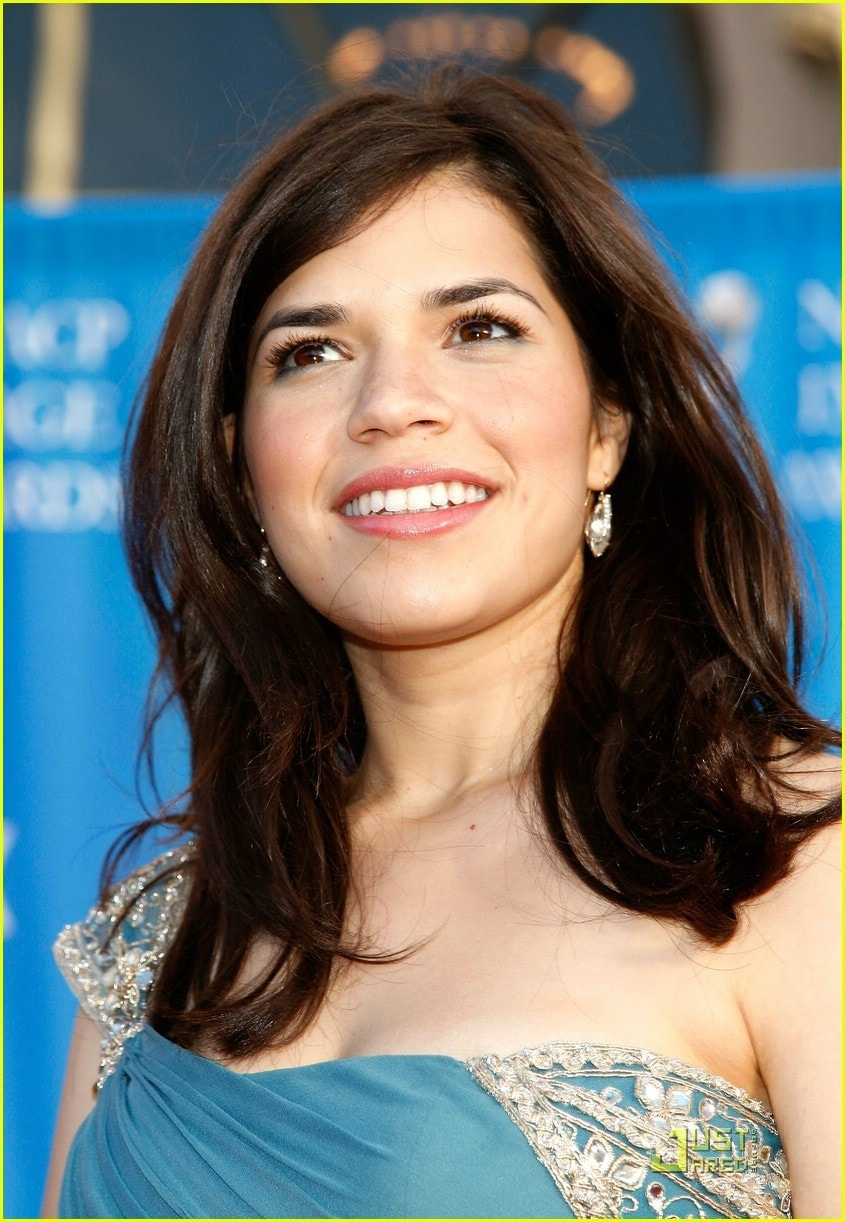
\includegraphics[width=.35\linewidth]{f1_ferrera4.jpg}
  \caption{Ferrera}
  \label{fig:sfig1}
\end{center}
\end{subfigure}
\begin{subfigure}{.33\textwidth}
\begin{center}
  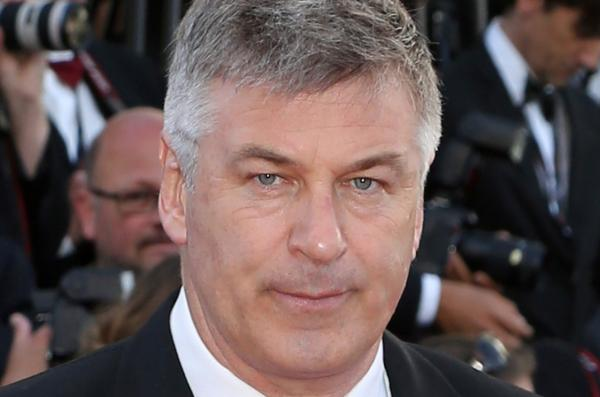
\includegraphics[width=.35\linewidth]{f2_baldwin24.jpg}
  \caption{Baldwin}
  \label{fig:sfig2}
\end{center}
\end{subfigure}
\begin{subfigure}{.33\textwidth}
\begin{center}
  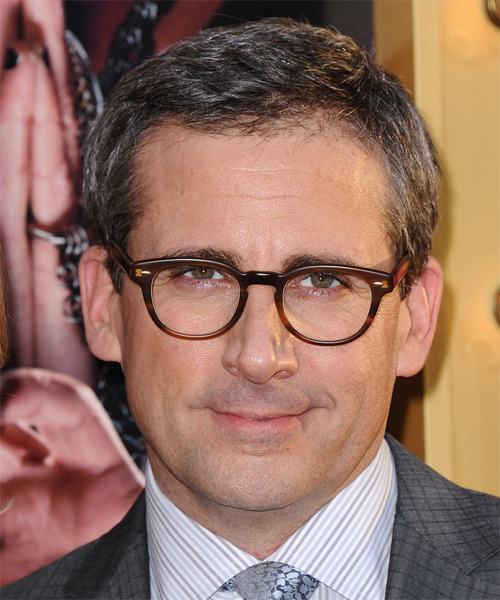
\includegraphics[width=.35\linewidth]{f3_carell164.jpg}
  \caption{Carell}
  \label{fig:sfig3}
\end{center}
\end{subfigure}
\begin{subfigure}{.33\textwidth}
\begin{center}
  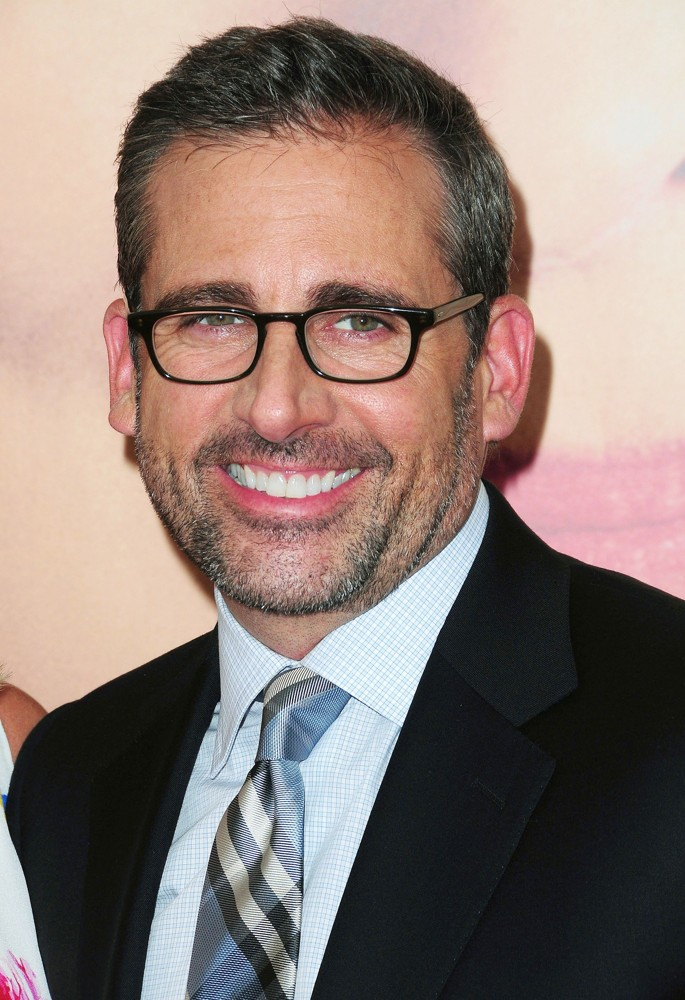
\includegraphics[width=.35\linewidth]{f4_carell11.jpg}
  \caption{Carell}
  \label{fig:sfig4}
\end{center}
\end{subfigure}
\begin{subfigure}{.33\textwidth}
\begin{center}
  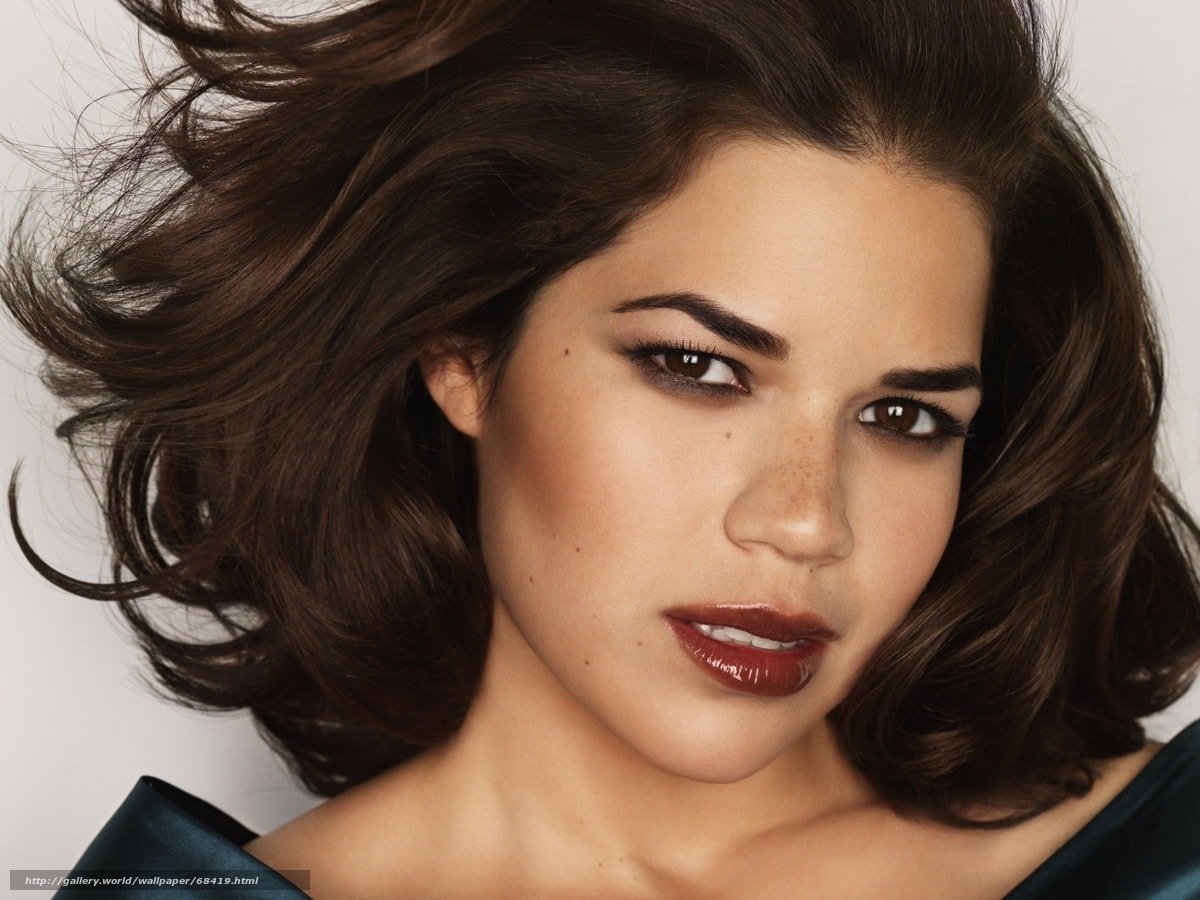
\includegraphics[width=.35\linewidth]{f5_ferrera128.jpg}
  \caption{Ferrera}
  \label{fig:sfig5}
\end{center}
\end{subfigure}
\begin{subfigure}{.33\textwidth}
\begin{center}
  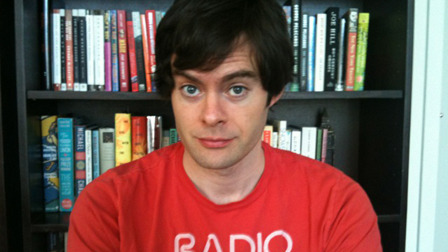
\includegraphics[width=.35\linewidth]{f6_hader20.jpg}
  \caption{Hader}
  \label{fig:sfig6}
\end{center}
\end{subfigure}
\caption{}
\end{figure*}

\textbf{Corresponding cropped out faces using the bounding box defined for the images:}
\begin{figure*}[!ht]
\begin{subfigure}{.33\textwidth}
\begin{center}
  
\includegraphics[width=.35\linewidth]{ff1_ferrera4.jpg}
  \caption{Ferrera}
  \label{fig:sfig1}
\end{center}
\end{subfigure}
\begin{subfigure}{.33\textwidth}
\begin{center}
  
\includegraphics[width=.35\linewidth]{ff2_baldwin24.jpg}
  \caption{Baldwin}
  \label{fig:sfig2}
\end{center}
\end{subfigure}
\begin{subfigure}{.33\textwidth}
\begin{center}
  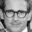
\includegraphics[width=.35\linewidth]{ff3_carell164.jpg}
  \caption{Carell}
  \label{fig:sfig3}
\end{center}
\end{subfigure}
\begin{subfigure}{.33\textwidth}
\begin{center}
  
\includegraphics[width=.35\linewidth]{ff4_carell11.jpg}
  \caption{Carell}
  \label{fig:sfig3}
\end{center}
\end{subfigure}
\begin{subfigure}{.33\textwidth}
\begin{center}
  
\includegraphics[width=.35\linewidth]{ff5_ferrera128.jpg}
  \caption{Ferrera}
  \label{fig:sfig3}
\end{center}
\end{subfigure}
\begin{subfigure}{.33\textwidth}
\begin{center}
  
\includegraphics[width=.35\linewidth]{ff6_hader20.jpg}
  \caption{Hader}
  \label{fig:sfig3}
\end{center}
\end{subfigure}
\caption{}
\end{figure*} \\
The defined rounding boxes are accurate for the majority of the images. Some exceptions are found in the example above. The bounding boxes for (b) Baldwin and (e) Ferrera did not cover their entire faces. These are bad samples and should not be used for analysis. \\
The cropped out faces are not well aligned because the actors show various facial expressions in their images.
\end{homeworkProblem}


%----------------------------------------------------------------------------------------
%	PART 2
%----------------------------------------------------------------------------------------
\begin{homeworkProblem}
From part 1, I already got a set of cropped faces stored in the directory \textit{cropped} by running the script \textit{get\_data\_and\_crop.py}. The format of all of the cropped images is [\textit{actor's last name}][\textit{download's order}], in which \textit{download's order} is the order that the original image was downloaded from the web. I therefore could distinguish the actor images using the file names. But I did not use the downloaded orders of the images to select the data, but instead wrote the script \textit{auto\_pick.py} that \textbf{randomly} picks a sample of 120 images for each of the actor. The first 100 images in the sample are  the training data, the next 10 images are the validation data, and the last 10 images are the test data. The script puts all training data into the folder \textit{part2\_data/train\_data}, all validation into the folder \textit{part2\_data/valid\_data} and all test data into the folder \textit{part2\_data/test\_data}. Both the scripts \textit{get\_data\_and\_crop.py} and \textit{auto\_pick.py} will be included in my submission.

\begin{figure*}[!ht]
\begin{center}
  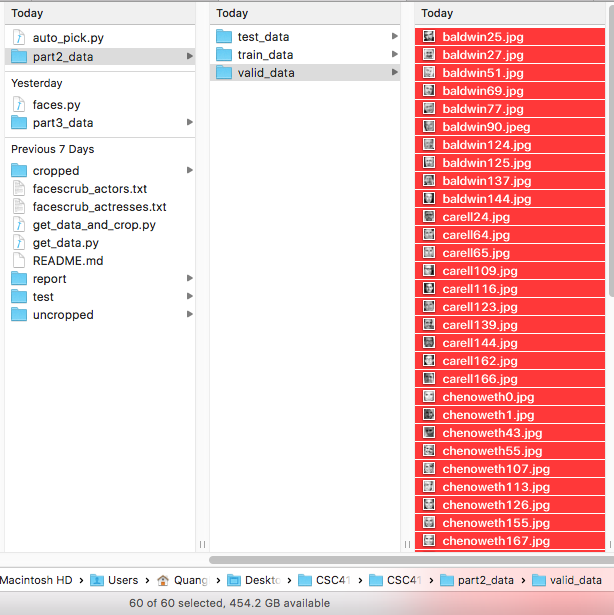
\includegraphics[width=0.5\linewidth]{auto_pick.png}
  \label{fig:sfig3}
\end{center}
\caption{60 randomly picked images of 6 actors in the validation set}
\end{figure*}

In the sets of images that I picked, few images were not well suited for doing analysis. They were images partitally show the faces of the actors or had inccorect bounding boxes. I replaced these images by other images that had not been picked. Note that because each actor has more than 120 images, there are always some spares that can be used as the substitution. Below are examples of types of images that should not be included.

\begin{figure*}[!ht]
\begin{center}
\begin{subfigure}{.4\textwidth}
\begin{center}
  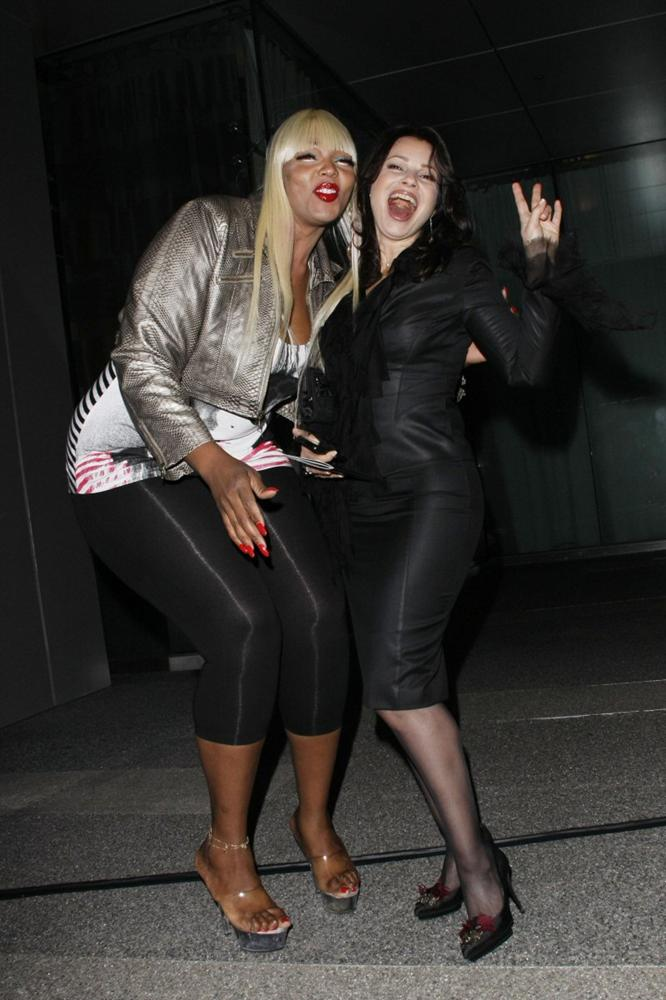
\includegraphics[width=.4\linewidth]{p2_drescher122.jpg}
  \label{fig:sfig3}
\end{center}
\caption{Original images}
\end{subfigure}
\begin{subfigure}{.4\textwidth}
\begin{center}
  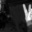
\includegraphics[width=.4\linewidth]{pp2_drescher122.jpg}
  \label{fig:sfig3}
\end{center}
\caption{Cropped images}
\end{subfigure}
\caption{Image with incorrect bounding box}
\end{center}
\end{figure*}

\begin{figure*}[!ht]
\begin{center}
\begin{subfigure}{.4\textwidth}
\begin{center}
  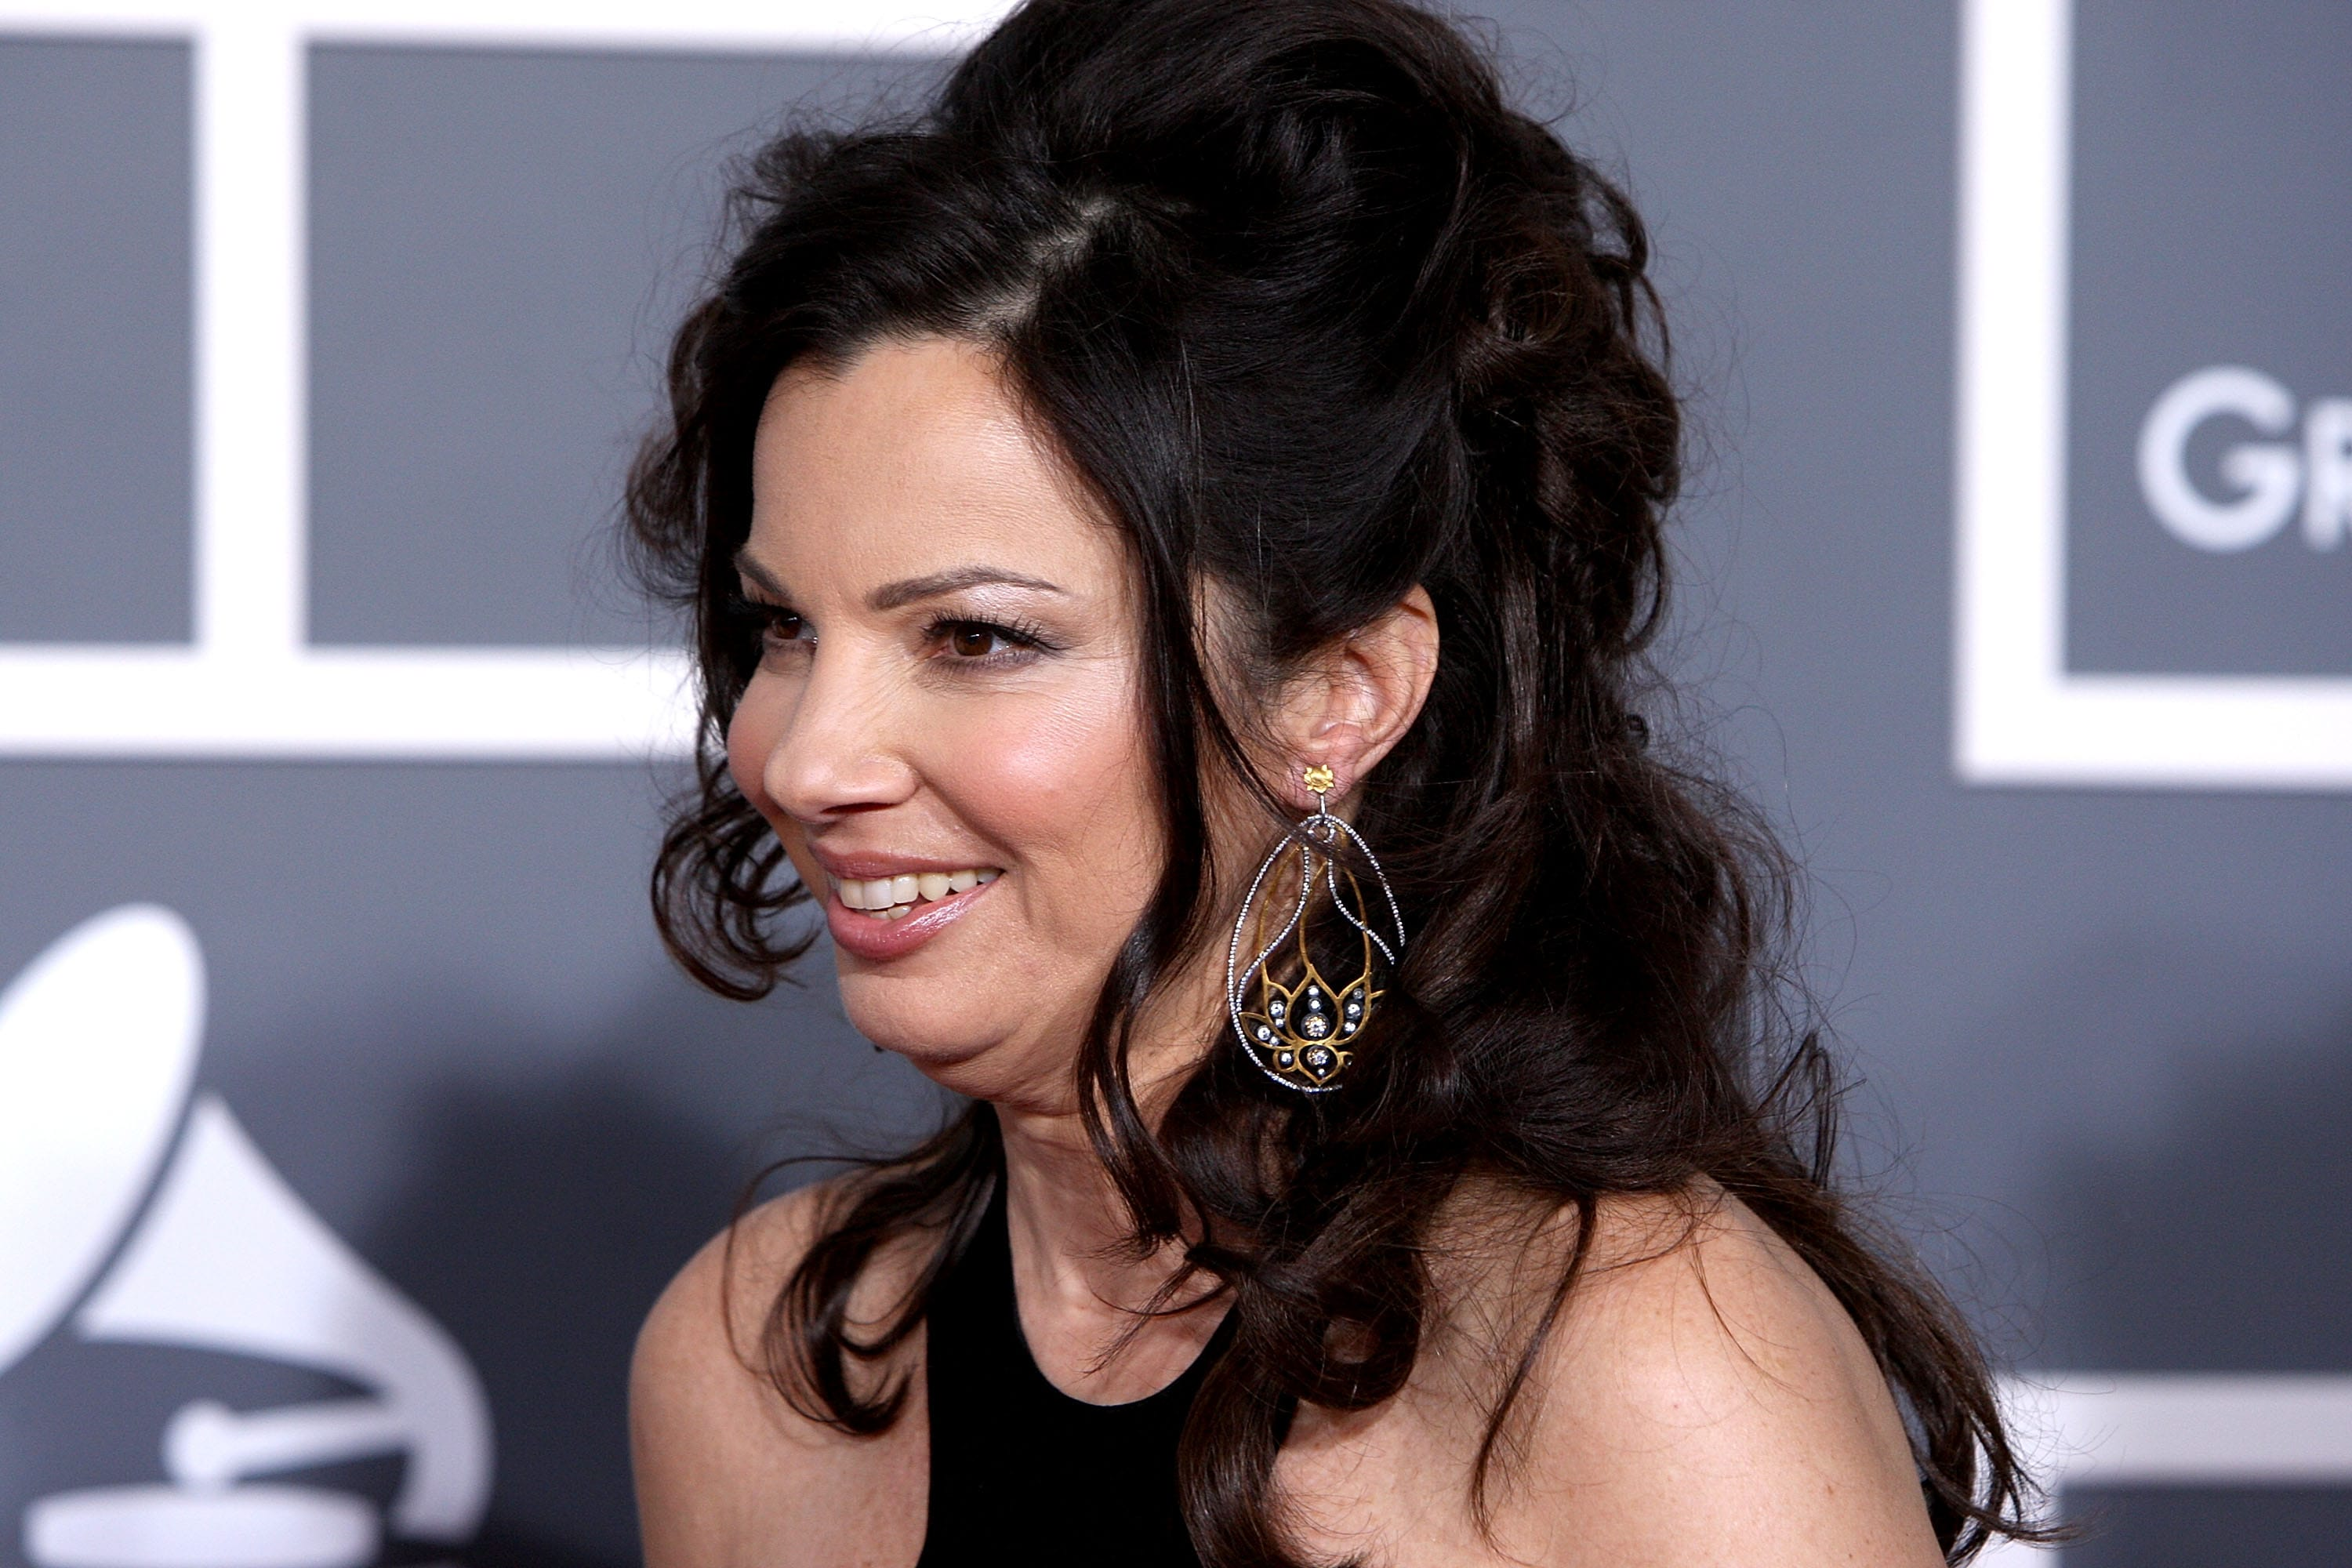
\includegraphics[width=.4\linewidth]{p2_drescher5.jpg}
\end{center}
\caption{Original images}
\end{subfigure}
\begin{subfigure}{.4\textwidth}
\begin{center}
  
\includegraphics[width=.4\linewidth]{pp2_drescher5.jpg}
\end{center}
\caption{Cropped images}
\end{subfigure}
\caption{Image shows only one side of the face}
\end{center}
\end{figure*} 

\begin{figure*}[!ht]
\begin{center}
\begin{subfigure}{.4\textwidth}
\begin{center}
  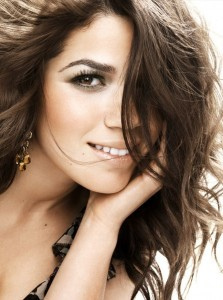
\includegraphics[width=.4\linewidth]{p2_ferrera165.jpg}
\end{center}
\caption{Original images}
\end{subfigure}
\begin{subfigure}{.4\textwidth}
\begin{center}
  
\includegraphics[width=.4\linewidth]{pp2_ferrera165.jpg}
\end{center}
\caption{Cropped images}
\end{subfigure}
\caption{Images show only one side of the face}
\end{center}
\end{figure*} 
\end{homeworkProblem}

\clearpage
%----------------------------------------------------------------------------------------
%	PART 3
%----------------------------------------------------------------------------------------
\begin{homeworkProblem}
\textbf{The cost function:} \\
\begin{equation}
f(x) = \dfrac{1}{2m} \sum_{i=1}^{m} (y^{(i)} - \theta^Tx^{(i)})
\end{equation}
Where
\begin{itemize}
\item $m$ is the sample's size.
\item x is a vector which stores the pixels of the images.
\item y is a vector with labels of the images (contains only 0s and 1s).
\end{itemize}

\textbf{Cost function and performance report:}
\begin{itemize}
\item The value of the cost function $f(x)$ for the \textbf{validation set} consisting 20 randomly picked images, 10 for each of the two actors is 0.02. 
The value of the cost function $f(x)$ for the \textbf{training set} consisting 200 randomly picked images, 100 for each of the two actors is also 0.02. 
\item The classifier was built using the test set with 100 randomly picked images for each of the two actors. 
\item The performance of the classifier on the \textbf{validation set} is 17 out of 20 images, a correctness of 85\%. 
\item The classifier correctlly identifies 97.5\% of the images in the \textbf{training set}. 
\item On the \textbf{test set} with 10 images for each actor, the classifier has a correctness rate of 90\%.
\end{itemize}

\textbf{Code to compute output of the classifier:}
\begin{lstlisting}[language=Python]
def classifier():
    #------------Building the classifier from training data-----------------#
    train_data = os.listdir("part3_data/train/")
    x = array([])
    y = zeros((200,), dtype=np.int)
    i = 0;
    train_size = 0;
    for name in train_data: 
        if "carell" in name or "hader" in name:
            train_size = train_size + 1;
            img = imread("part3_data/train/" + name)
            img = rgb2gray(img)
            img = img.flatten()
            if x.size == 0:
                x = vstack([img])
            elif x.size > 0:
                x = vstack([x, img])
            if "hader" in name:
                y[i] = 1
            
            i = i + 1;
    x = x.T
    theta0 = np.zeros(1025)
    theta = grad_descent(f, df, x, y, theta0, 0.000001, train_size)
    
    
    #--------------Running the classifier to obtain the result---------------#
    test_data = os.listdir("part3_data/test/");
    count_hader = 0; # Number of correct classification for hader.
    count_carell = 0; # Number of correct classification for carell.
    test_size = 0;
    for name in test_data:
        if "carell" in name or "hader" in name:
            test_size = test_size + 1;
            imgtest = imread("part3_data/test/" + name)
            imgtest = rgb2gray(imgtest)
            imgtest = imgtest.flatten()
            result = dot(theta[1:], imgtest) + theta[0] # Hypotheis result
            # print("Hypothesis result: ", result)
            if result > 0.5:
                print('The image {} is classified to be {}'.format(name,'Bill Hader'))
                if "hader" in name: # classification result matches the label
                    count_hader = count_hader + 1;.
            elif result <= 0.5:
                print('The image {} is classified to be {}'.format(name,'Steve Carell'))
                if "carell" in name: # classification result matches the label
                    count_carell = count_carell + 1;
    print(float(count_hader + count_carell)/test_size)*100; # Percentage result
\end{lstlisting}
To build the classifier, y is set to 1 if the image is of actor Bill Hader, and 0 if the image is of actor Steve Carell. Gradient descent algorithm is then used to find the $\theta$. The classifier do the classification based on the value returned by the hypothesis function $h(x)=\theta^Tx$. If the result is $>0.5$ the image is classified to be of Bill Hader, else if the result is $<0.5$, the image is classified to be of Steve Carell. The full code can be found in the faces.py \\

\textbf{Things I considered:} \\
To make the algorithm works, I need an $\alpha$ level that is neither too big or too small. $\alpha$ as defined in class is the step size used in gradient descent algorithm to find the local minimum. We don't want $\alpha$ to be too small, because it would take too many iterations to reach the local minimum. In constrast, if the step size is too big, the algorithm would bypass the optimal point, and diverge to infinity. I also need an intital theta, which is sufficiently small. The inital theta was set to be a vector with only zeros.\\

Each gray scale images is represented by a numby array in 2-D, but the atrix x in the cost function $f(x)$ only takes 1-D vector for each training sample. So I have to flatten the image by combining all rows in the matrices into one single row, forming a new 1-D vector. This is done by calling \textit{img.flatten()}.

\clearpage
\end{homeworkProblem}
%----------------------------------------------------------------------------------------
%	PART 4
%----------------------------------------------------------------------------------------
\begin{homeworkProblem}

\begin{figure*}[!ht]
\begin{center}
  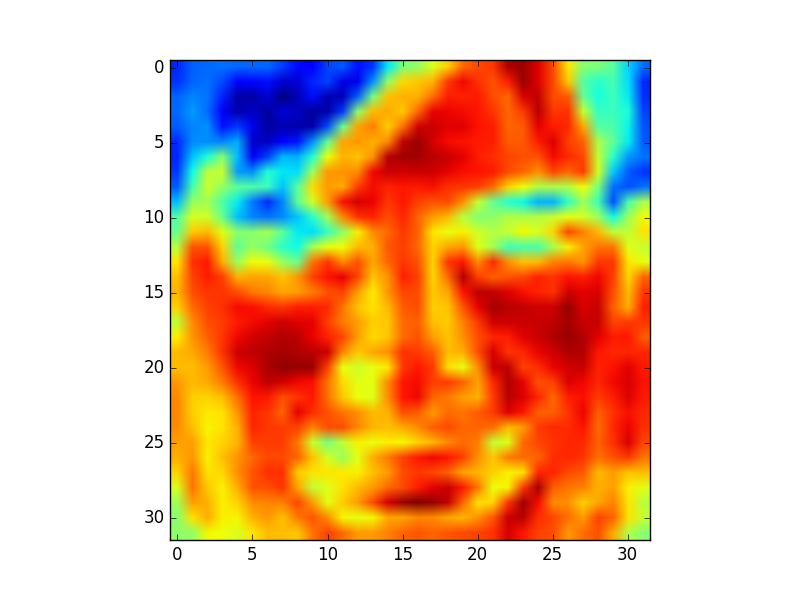
\includegraphics[width=0.5\linewidth]{part4_2each.png}
  \label{fig:sfig3}
\end{center}
\caption{The \textit{theta} image built using a training set contains 4 images, 2 for each of the two actors Steve Carell and Bill Hander.}
\end{figure*}

\begin{figure*}[!ht]
\begin{center}
  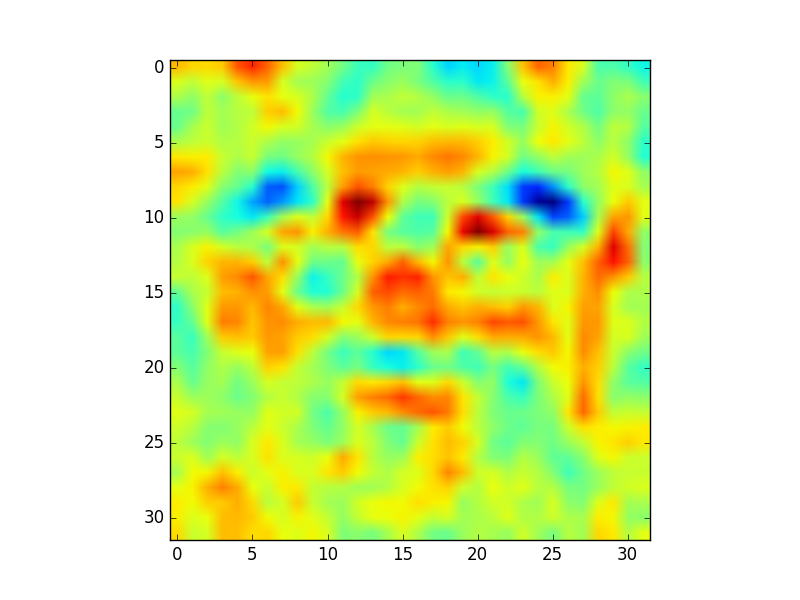
\includegraphics[width=0.5\linewidth]{part4_100each.png}
  \label{fig:sfig3}
\end{center}
\caption{The \textit{theta} image built using a training set contains 200 images, 100 for each of the two actors Steve Carell and Bill Hander.}
\end{figure*}
\end{homeworkProblem}
\clearpage
%----------------------------------------------------------------------------------------
%	PART 5
%----------------------------------------------------------------------------------------
\begin{homeworkProblem}
\textbf{Picking the data:} \\
I created a new script \textit{auto\_pick\_part5.py} that automatically pick a train set, a validation set and a test set of the sizes I specified. This is the more advanced version of \textit{auto\_pick.py} that I created in Part 2. Below is the signature of the function in the script used to pick the images. \\
\begin{lstlisting}[language=Python]
def pickrandom_p5(actor, source_dir, training_dir, valid_dir, test_dir,
                    train_size, valid_size, test_size):
\end{lstlisting}
Where: 
\begin{itemize}
\item \textbf{actor}: is the list of actor to be picked from.
\item \textbf{source\_dir}: is the source directory path of th images to be picked from.
\item \textbf{training\_dir}, \textbf{valid\_dir}, \textbf{test\_dir} are path to the destination for the training, validation and test sets respectively.
\item \textbf{train\_size}, \textbf{valid\_size}, \textbf{test\_size} are sizes of the training, validation and test sets respectively (number of images per actor in the set).
\end{itemize}
For instance, to randomly pick a training set that has 10 images for each of the actors from the cropped images stored in folder \textit{cropped/}, we do 
\begin{lstlisting}[language=Python]
pickrandom_p5(act, "cropped/", "part5_data/train_data_10", "", "", 10, 0, 0); \\
\end{lstlisting}  
\textbf{Plot the performance of the classifiers on the training and validation sets:}
The code for this part can be found in \textit{faces.py}. I built the the classifiers using different training set size and recorded the performance of the classifiers on the training and validation sets. The table below shows the recorded data.
\begin{center}
\begin{tabular}{| l |l | l | p{5cm}|}
\hline
\textbf{Training set size} & \textbf{Performance on the training set (\%) }& \textbf{ Performance on the validation set (\%)} \\ \hline
2 & 66.67 & 61.66 \\ \hline
5 & 83.30 & 58.33 \\ \hline
10 & 93.33 & 70.00 \\ \hline
20 & 95.60 & 88.30 \\ \hline
30 & 97.70 & 75.50 \\ \hline
40 & 97.50 & 85.00 \\ \hline
50 & 97.33 & 95.00 \\ \hline
60 & 98.05 & 93.33 \\ \hline
70 & 98.10 & 86.67 \\ \hline
80 & 98.30 & 90.00 \\ 
\hline
\end{tabular}
\end{center}
I then used the data to plot a graph that demonstrates the result of overfitting, that is building a classifier that works well on training data but does not work equally well on unseen data. Note that the training set size is the number of images for each actor in the set.
\clearpage
\begin{figure*}[!ht]
\begin{center}
  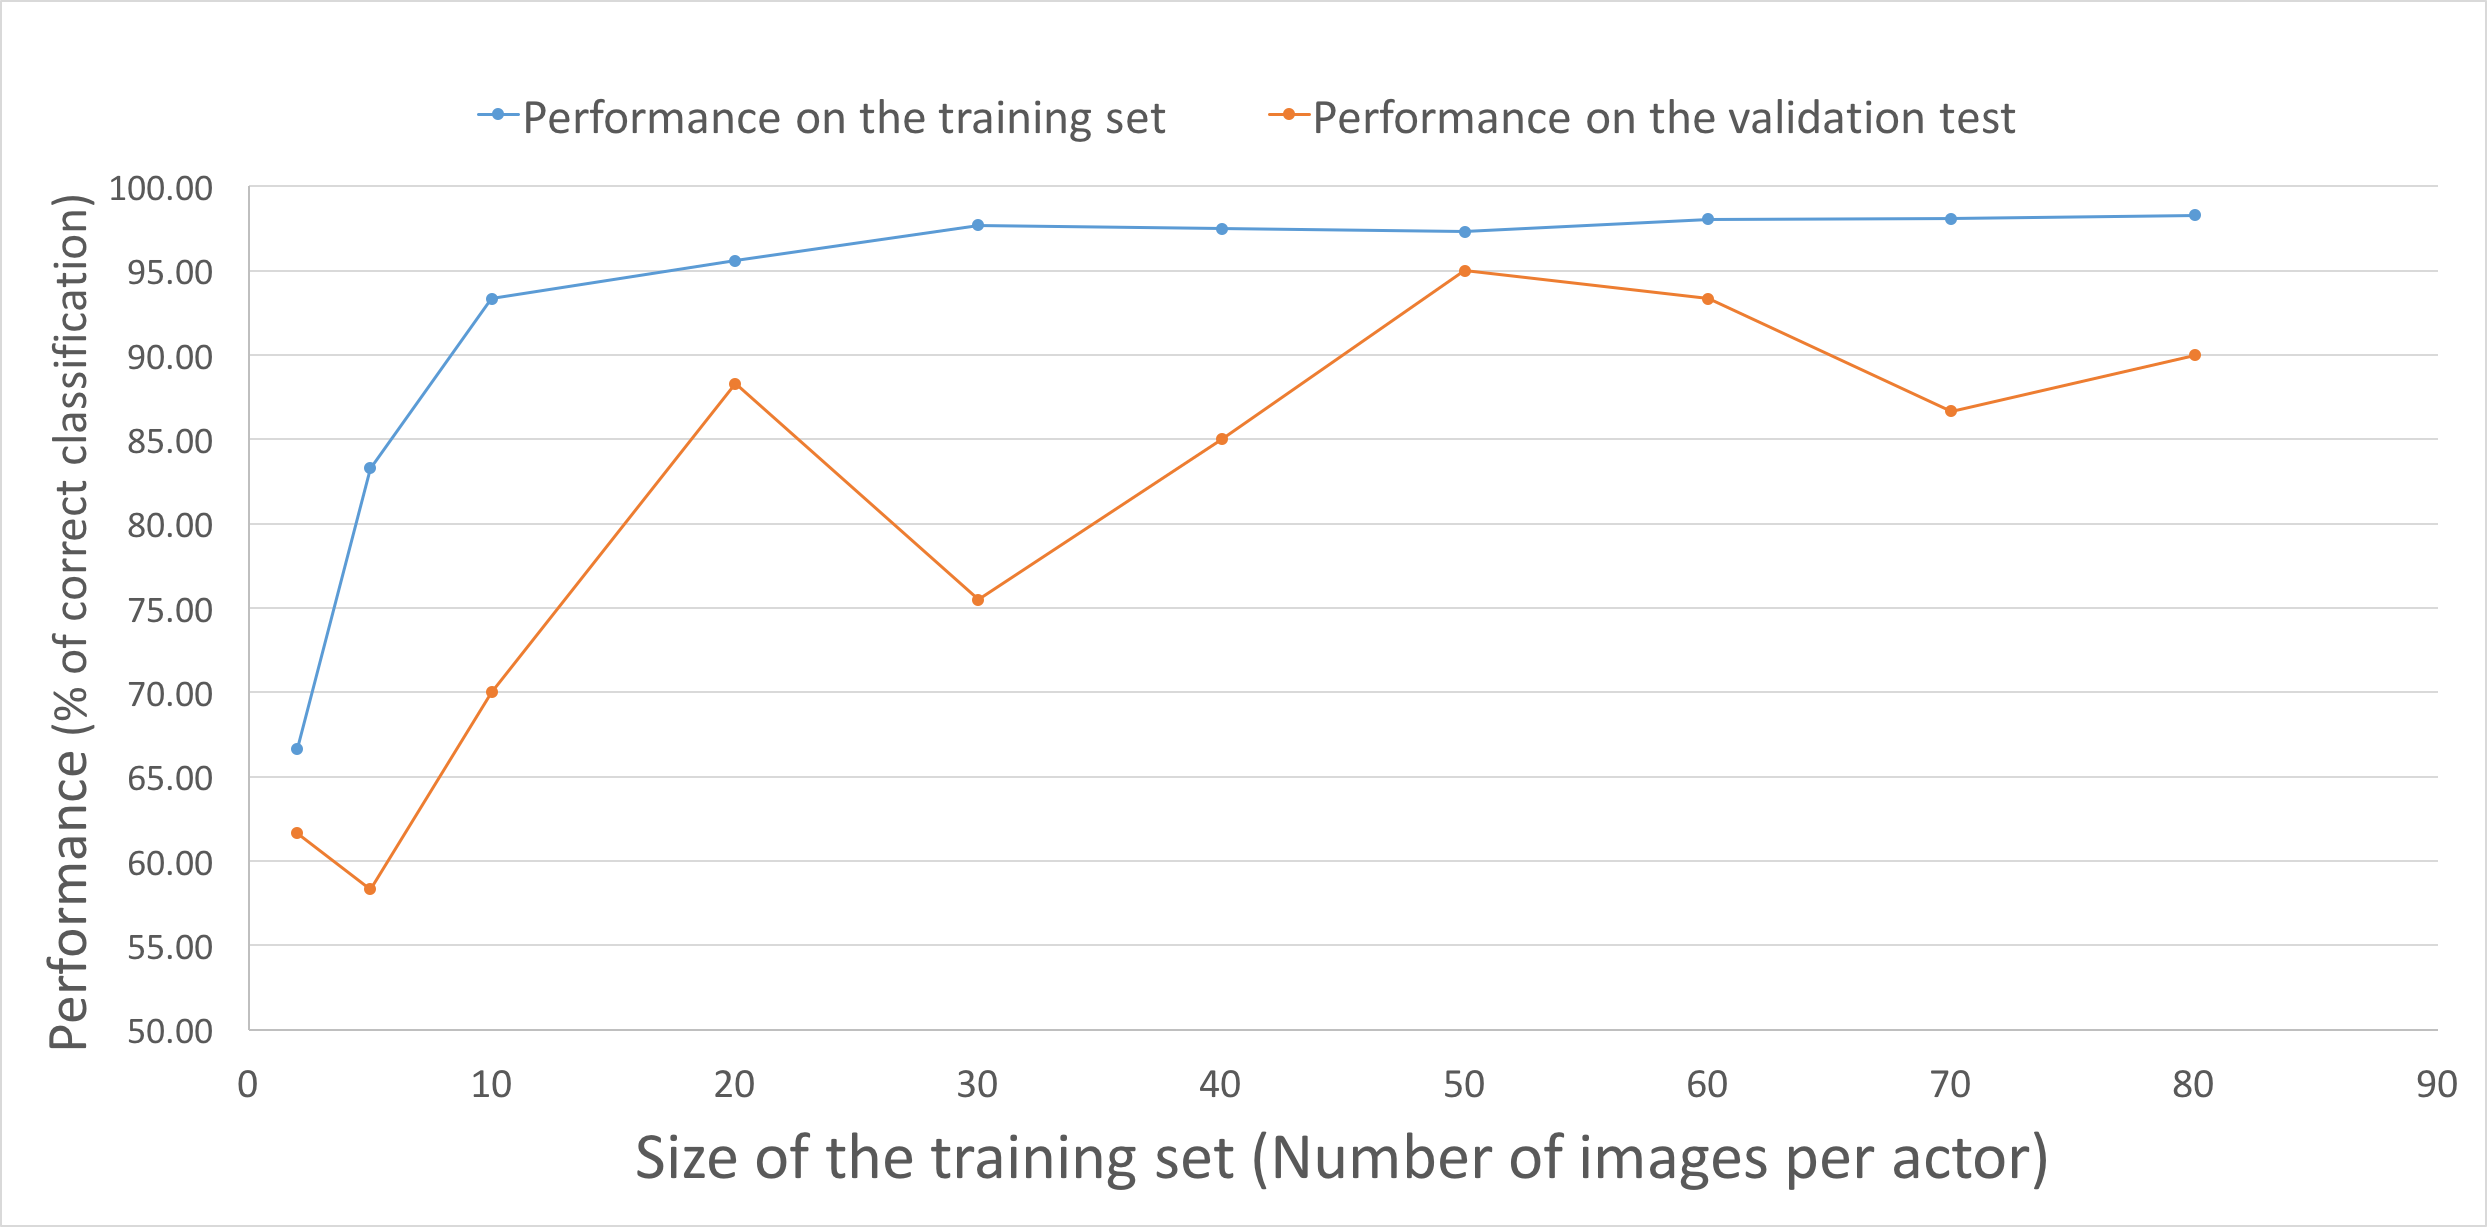
\includegraphics[width=1.0\linewidth]{part5_plot.png}
  \label{fig:sfig3}
\end{center}
\caption{The performance on the training data is always better than on the validation data. However, the performance gap decreases as the the size of the training samples increases. When the training size increases from 20 to 30 images per actor, the peformance on the training set increases whereas the performance on the validation set decreases, an indication that overfitting has happened.}
\end{figure*}
\textbf{Performance of the classifier on actors in act\_test} \\
I modified the script \textit{get\_data\_and\_crop\.py} created in part 1, to download images of the actors in \textit{act\_test} and do face cropping.There were only minor modifications on the names of the destination folders and the list of name of actors to be download. I saved the modified version with the new name \textit{get\_data\_and\_crop\_part5.py}, just in case you want to reproduce the data. \\
I ran the classifier with the training set of size 70 created in the first part on the entire set of cropped images of the actors in \textit{act\_test}. The correctness rate was 85.74 \%, a 10 \% lower than the performance of the classifier on \textit{act}.
\end{homeworkProblem}
\clearpage
\begin{homeworkProblem}
\subsection{(a)}
We have $\theta_{pq} = \theta_{qp}^T$, so we have the following equality: \\
\[
\sum_{i}^m(\sum_{j}^k(\theta^Tx^{(i)} - y^{(i)})^2_j)
=
\sum_{i}^m\sum_{j}^k
\left(
\begin{bmatrix}
    \theta_{11}^{T} & \dots & \dots & \dots &\theta_{1n}^{T} \\
    \vdots & \ddots & \vdots & \vdots & \vdots\\
    \vdots & \vdots & \theta_{qp}^{T} & \vdots & \vdots\\ 
    \vdots & \vdots & \vdots & \ddots & \vdots\\
    \theta_{k1}^{T} & \dots & \dots & \dots & \theta_{kn}^{T}
\end{bmatrix}
\times
\begin{bmatrix}
    x_{1}^{(i)}  \\
    \vdots \\
    x_{p}^{(i)}  \\
    \vdots  \\
    x_{n}^{(i)} 
\end{bmatrix}
-
\begin{bmatrix}
    y_{1}^{(i)}  \\
    \vdots  \\
    y_{q}^{(i)}  \\
    \vdots  \\
    y_{k}^{(i)} 
\end{bmatrix}
\right)^2_{j}
\]
Because we are doing paritial deriative for $\theta_{pq} = \theta_{qp}^T$, we only need to take the deriative of the component where $\theta_{qp}^T$ presents.
\begin{equation}
\begin{split}
\dfrac{dJ}{d\theta_{pq}} \sum_{i}^m(\sum_{j}^k(\theta^Tx^{(i)} - y^{(i)})^2_j) & = \dfrac{dJ}{d\theta_{qp}^T} \sum_{i}^m(\sum_{j}^k(\theta^Tx^{(i)} - y^{(i)})^2_j)\\
& = \sum_{i}^m\dfrac{d}{d\theta_{qp}^T}(\theta_{q1}^Tx_{1}^{(i)} + \theta_{q1}^Tx_{1}^{(i)} + \theta_{q2}^Tx_{2}^{(i)} + ... + \theta_{qp}^Tx_{p}^{(i)} + ... + \theta_{qn}^Tx_{n}^{(i)} - y^{(i)}_q)^{2} \\
& = 2\sum_{i}^m(x_p^{(i)}(\theta_{q1}^Tx_{1}^{(i)} + \theta_{q1}^Tx_{1}^{(i)} + \theta_{q2}^Tx_{2}^{(i)} + ... + \theta_{qp}^Tx_{p}^{(i)} + ... + \theta_{qn}^Tx_{n}^{(i)} - y^{(i)}_q))\\
& = 2\sum_{i}^m x_p^{(i)}(\theta^T_q x^{(i)} - y_q^{(i)})
 \end{split}
\end{equation}
This function is verified to be correct in part (d). 
\subsection{(b)}
\[
\dfrac{dJ}{d\theta} = 
\begin{bmatrix}
    \dfrac{dJ}{d\theta_{11}^{T}} & \dots & \dots & \dots &\dfrac{dJ}{d\theta_{1n}^{T}} \\
    \vdots & \vdots & \vdots & \vdots & \vdots\\ 
    \vdots & \vdots & \vdots & \vdots & \vdots\\
    \dfrac{dJ}{d\theta_{k1}^{T}} & \dots & \dots & \dots & \dfrac{dJ}{d\theta_{kn}^{T}}
\end{bmatrix} \\
= 
\begin{bmatrix}
    2\sum_{i}^m x_1^{(i)}(\theta^T_1 x^{(i)} - y_1^{(i)}) & \dots & \dots & \dots & 2\sum_{i}^m x_n^{(i)}(\theta^T_1 x^{(i)} - y_1^{(i)}) \\
    \vdots & \vdots & \vdots & \vdots & \vdots\\ 
    \vdots & \vdots & \vdots & \vdots & \vdots\\
    2\sum_{i}^m x_1^{(i)}(\theta^T_k x^{(i)} - y_k^{(i)}) & \dots & \dots & \dots & 2\sum_{i}^m x_n^{(i)}(\theta^T_k x^{(i)} - y_k^{(i)})
\end{bmatrix}
\]
\[
= 2
\begin{bmatrix}
    x_1^{(1)} & x_1^{(2)} & \dots & \dots & x_1^{(m)} \\
    \vdots & \vdots & \vdots & \vdots & \vdots\\ 
    \vdots & \vdots & \vdots & \vdots & \vdots\\
    x_n^{(1)} & x_n^{(2)} & \dots & \dots & x_n^{(m)} \\
\end{bmatrix} \\
\times 
\begin{bmatrix}
    \sum_{i}^m (\theta^T_1 x^{(i)} - y_1^{(i)}) & \dots & \dots & \dots & \sum_{i}^m (\theta^T_1 x^{(i)} - y_1^{(i)}) \\
    \vdots & \vdots & \vdots & \vdots & \vdots\\ 
    \vdots & \vdots & \vdots & \vdots & \vdots\\
    \sum_{i}^m (\theta^T_k x^{(i)} - y_k^{(i)}) & \dots & \dots & \dots & \sum_{i}^m (\theta^T_k x^{(i)} - y_k^{(i)})
\end{bmatrix}^T
\]
\[
= 2X
\times 
\begin{bmatrix}
    (\theta^T_1 x^{(1)} - y_1^{(1)}) + \dots + (\theta^T_1 x^{(m)} - y_1^{(m)}) & \dots & \dots & \dots & \theta^T_1 x^{(1)} - y_1^{(1)}) + \dots +  \theta^T_1 x^{(m)} - y_1^{(m)}) \\
    \vdots & \vdots & \vdots & \vdots & \vdots\\ 
    \vdots & \vdots & \vdots & \vdots & \vdots\\
    (\theta^T_k x^{(1)} - y_k^{(1)}) + \dots + (\theta^T_k x^{(m)} - y_k^{(m)}) + & \dots & \dots & \dots & (\theta^T_k x^{(1)} - y_k^{(1)}) + \dots + (\theta^T_k x^{(m)} - y_k^{(m)})
\end{bmatrix}^T
\]
\begin{equation}
= 2X(\theta^{T}X - Y)^{T}
\end{equation}
Where
\begin{itemize}
\item $\theta$ is an $n \times k$ matrix, in which $n$ is the number of pixels in an images plus $1$ (1025), and $k$ is the number of possible labels. Then $\theta^{T}$ is a matrix of size $k \times n$.
\item $X$ is the input matrix of size $n \times m$, $n$ again is the number of pixels plus 1 (1025), and $m$ is the size of the training samples.
\item $Y$ is the output label matrix of size $k \times m$, that is the number of availables labels $\times$ the size of the training samples.
\item $\theta^{T}X$ is the hypothesis matrix of size $k \times m$. Therefore, $\theta^{T}X - Y$ also has size $k \times m$.
\item $2X$ has size $n \times m$, multiplying by the $m \times k$ matrix $(\theta^{T}X - Y)^T$ generate the cost matrix $2X(\theta^{T}X-Y)^T$ that has size $n \times k$.
\end{itemize}
\subsection{(c)}
\textbf{Vectorized gradient function:}
\begin{lstlisting}[language=Python]
def vectorized_gradient(x, y, theta):
    x = vstack((ones((1, x.shape[1])), x))
    return dot(dot(2,x), (dot(theta.T, x) - y).T)
\end{lstlisting}

\textbf{Cost function:}
\begin{lstlisting}[language=Python]
def cf_part6(x, y, theta):
    x = vstack((ones((1, x.shape[1])), x))
    return sum((dot(theta.T,x) - y) ** 2)
\end{lstlisting}

\subsection{(d)}
\textbf{Gradient Component Function:} The \textit{finite\_difference\_gradient} function below takes in the matrices x, y and theta, it computes the component (p, q) of the gradient of the cost function. This function is the code implementation of the gradient formula derived in part (a). \\\\
\begin{lstlisting}[language=Python]
# Computing the component (p, q) of the gradient matrix. 
def finite_difference_gradient(x, y, theta, p, q):
    x = vstack((ones((1, x.shape[1])), x))
    sum = 0;
    for i in range(x.shape[1]):
        sum = sum + x[p][i] * (dot(theta.T[q],x[:,i]) - y[q][i]);
    return 2 * sum;
\end{lstlisting}
\textbf{Testing:}  I create two matrices x and y, compute the gradient using both methods, and compare if the two results are the same.
\begin{lstlisting}[language=Python]
def test_part6():
    # Say each images has 5 pixels (not include 1 on top)
    # 2 images [1,1, 1, 1,5] ,[2, 1, 1, 1, 1]
    # 3 possible labels [1, 0, 0], [0, 1, 0], [0, 0, 1]
    # x = (5 + 1) x 2 matrix
    # y = 3 x 2 matrix
    # theta.T = 3 x (5 + 1) matrix
    
    # Form an x
    img1 = array([1,1, 1, 1,5])
    img2 = array([2, 1, 1, 1, 1])
    img = vstack([img1, img2])
    x = img.T # x is in n * m, where n is number of pixels and m is number of samples.
    print("------ x is (without 1 on top yet) -------")
    print(x)
    
    # Form a theta
    theta0 = zeros((6, 3))
    print("----------- theta zero is -------------")
    print(theta0) # theta is in n * k, where n is number of pixels and k is number of labels..
    
    # Form a y
    y = array([[1, 0, 0], [0, 0, 1]]);
    y = y.T; # y is in k * m, where k is number of labels and m is the sample size.
    print("---------------- y is -----------------")
    print(y)
    
    print("---------vectorized gradient-----------")
    print(vectorized_gradient(x, y, theta0))
    
    print("------gradient computed using finite diffeence------")
    g = zeros_like(vectorized_gradient(x, y, theta0))
    
    # Compute every componento f the gradient using fitenite difference method.
    for p in range(x.shape[0] + 1):
        for q in range(y.shape[0]):
            g[p, q] = finite_difference_gradient(x, y, theta0, p, q)
    print(g)
\end{lstlisting}
\textbf{Output:}
\begin{lstlisting}[language=Python]
------------- x is (without 1 on top yet) ---------------
[[1 2]
 [1 1]
 [1 1]
 [1 1]
 [5 1]]
----------- theta zero is -------------
[[ 0.  0.  0.]
 [ 0.  0.  0.]
 [ 0.  0.  0.]
 [ 0.  0.  0.]
 [ 0.  0.  0.]
 [ 0.  0.  0.]]
---------------- y is -----------------
[[1 0]
 [0 0]
 [0 1]]
---------vectorized gradient-----------
[[ -2.   0.  -2.]
 [ -2.   0.  -4.]
 [ -2.   0.  -2.]
 [ -2.   0.  -2.]
 [ -2.   0.  -2.]
 [-10.   0.  -2.]]
------gradient computed using finite diffeence------
[[ -2.   0.  -2.]
 [ -2.   0.  -4.]
 [ -2.   0.  -2.]
 [ -2.   0.  -2.]
 [ -2.   0.  -2.]
 [-10.   0.  -2.]]
\end{lstlisting}
\textbf{Conclusion}: There is no difference between the gradient matrices computed using the two techniques. Therefore, the deriative function derived in part (a) is verified.

\clearpage
\end{homeworkProblem}
\begin{homeworkProblem}
\textbf{Codes:} \\
The code for this part can be found in \textit{faces.py} and \textit{auto\_pick\_part5.py}. \\\\
\textbf{Picking The Data:} \\
I used the script \textit{auto\_pick\_part5.py} (created in part 5) to randomly select 100 training images and 10 validating images for every actor from the folder cropped that stores all cropped images of the actors. So in total, I have 600 images in the training set, and 60 images in the validation set. \\\\
\textbf{Classifier:} \\
I set $\theta_{initial}$ to be a zero matrix of size $n \times k$. The step size $\alpha$ for the gradient descent algorithm was set to be $10^{-6}$, this was the result of a trial and error process. I tried with bigger $\alpha$ $10^{-5}$, $10^{-4}$, but this resulted in NaN values returned by the computation for some components for theta. It was because the large step size caused some gradient matrix's compoenents to bypass their local minimums and diverge. Else if I got $\alpha$ set to smaller numbers, like $10^{-7}$ or $10^{-8}$, gradient descent took huge number of iterations to give a decent correctness rate.\\

With the step size $\alpha = 10^{-6}$ and $max number of iterations = 50000$ for the gradient descent algorithm, the classifier gives the correctness rate of $99.3 \%$ for the training set and $93.3 \%$ for the validation test. Because of the large number of iterations, you may have to wait few minutes before the program finishes executing. 
\end{homeworkProblem}

\clearpage
\begin{homeworkProblem}
\textbf{Codes:} The code for this part is in \textit{faces.py}.\\
\textbf{Images:} \\
\begin{figure*}[!ht]
\begin{subfigure}{.55\textwidth}
\begin{center}
  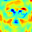
\includegraphics[width=.55\linewidth]{part8_carell.png}
  \caption{Steve Carell}
\end{center}

\end{subfigure}
\begin{subfigure}{.55\textwidth}
\begin{center}
  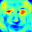
\includegraphics[width=.55\linewidth]{part8_baldwin.png}
  \caption{Alec Baldwin}
\end{center}
\end{subfigure} 

\begin{subfigure}{.55\textwidth}
\begin{center}
  
\includegraphics[width=.55\linewidth]{part8_hader.png}
  \caption{Bill Hader}
\end{center}

\end{subfigure} 
\begin{subfigure}{.55\textwidth}
\begin{center}
  
\includegraphics[width=.55\linewidth]{part8_chenoweth.png}
  \caption{Kristin Chenoweth}
\end{center}

\end{subfigure}
\begin{subfigure}{.55\textwidth}
\begin{center}
  
\includegraphics[width=.55\linewidth]{part8_ferrera.png}
  \caption{America Ferrera}
\end{center}

\end{subfigure}
\begin{subfigure}{.55\textwidth}
\begin{center}
  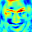
\includegraphics[width=.55\linewidth]{part8_drescher.png}
  \caption{Fran Drescher}
\end{center}

\end{subfigure}
\end{figure*}
\end{homeworkProblem}

\end{document}
